%% Overleaf			
%% Software Manual and Technical Document Template	
%% 									
%% This provides an example of a software manual created in Overleaf.

\documentclass{ol-softwaremanual}

% Packages used in this example
\usepackage{graphicx}  % for including images
\usepackage{microtype} % for typographical enhancements
\usepackage{minted}    % for code listings
\usepackage{amsmath}   % for equations and mathematics
\setminted{style=friendly,fontsize=\small}
\renewcommand{\listoflistingscaption}{List of Acronyms}
\usepackage{hyperref}  % for hyperlinks
\usepackage[a4paper,top=4.2cm,bottom=4.2cm,left=3.5cm,right=3.5cm]{geometry} % for setting page size and margins

% Add in the preamble
\usepackage{array}
\usepackage{graphicx}

\usepackage{booktabs} 
\usepackage{array}
\usepackage{longtable}
\usepackage{booktabs}
\usepackage{array}
\usepackage{gensymb}


\usepackage{ragged2e}

\usepackage{subcaption}
\renewcommand{\thesubfigure}{\thefigure\alph{subfigure}}

\usepackage{float}
\usepackage{subcaption}

% Custom macros used in this example document
\newcommand{\doclink}[2]{\href{#1}{#2}\footnote{\url{#1}}}
\newcommand{\cs}[1]{\texttt{\textbackslash #1}}

% Frontmatter data; appears on title page
\title{Analysis of Tritium with the PEM system}
\version{1}
\author{Eawag}
%\softwarelogo{\includegraphics[width=8cm]{}}

\begin{document}

\maketitle

\tableofcontents
\newpage

\section*{List of Acronyms}

\renewcommand{\arraystretch}{1.5}

\begin{tabular}{@{}p{2.2cm}p{10cm}@{}}
\textbf{PEM}  & Proton Exchange Membrane \\

\textbf{PTFE} & Polytetrafluoroethylene \\

\textbf{LSC}  & Liquid Scintillation Counting \\

\textbf{MEA}  & Membrane Electrode Assembly \\
\end{tabular}

\newpage
\section{Introduction}

 

\section{Assembly of the Electrolytic cell}


\subsection{Materials Checklist}
The list of materials required to assemble a PEM electrolytic cell is given ~\href{https://github.com/brennmat/pemPy/tree/main/handbook/Materials%20list}{here}.

 \subsection{The Sandwich}

\subsubsection*{Assembly of the sandwich}
The bottom holder has two openings for the electrical terminals,
one near the centre and the other towards the outer edge.

\begin{itemize}

    \item Insert the shorter terminal (negative) through the
    opening near the centre and carefully bend the wire around
    the region where the MEA will be positioned.

    \item Insert the longer terminal (positive) through the
    outer opening.

    \item Apply glue around the head of each terminal to
    seal it to the holder.

    \item Leave the holder for approximately 48 hours
    to allow the adhesive to cure.
\end{itemize}

 
 \begin{figure}[H]
    \centering

    \begin{subfigure}{0.45\textwidth}
        \centering
        \includegraphics[width=\linewidth]{20260813_130249.jpg}
        \caption{Thread of the terminal lightly covered in glue being attached to holder}
        \label{fig:1s1}
    \end{subfigure}
    \hfill
    \begin{subfigure}{0.45\textwidth}
        \centering
        \includegraphics[width=\linewidth]{20260813_125555.jpg}
        \caption{Anode and Cathode terminals attached to the holder}
        \label{fig:1s2}
    \end{subfigure}
\end{figure}



\begin{itemize}
    \item Attach the mounting ring to the bottom holder after the adhesive has cured.

    \item Place the assembly on a stand in a room-temperature water bath, ensuring it is fully submerged.

    \item Gently tap the holder to remove trapped air bubbles. Repeat as necessary throughout the assembly.

    \item Place the gold mesh current collector on the bottom holder, ensuring electrical contact with the cathode terminal.

    \item Position the seal ring on the holder.
\end{itemize}


\begin{figure}[H]
    \centering
   
    \begin{subfigure}{0.45\textwidth}
    \includegraphics[width=\linewidth]{20260819_101242.jpg}
    \caption{Holder submerged on a water jug}
    \label{fig:s3}
     \end{subfigure}
 \hfill
\begin{subfigure}{0.45\textwidth}
    \includegraphics[width=\linewidth]{20260819_101815.jpg}
    \caption{Gold mesh current collector placed on the submerged holder}
    \label{fig:s4}
\end{subfigure}

     
\end{figure}
\begin{itemize}
    \item Place the cathode on the gold mesh current collector, with its rougher surface facing downwards towards the mesh.

    \item Place the Nafion membrane directly on top of the cathode.

    \item Place the anode on the membrane, with its smoother surface facing downwards towards the membrane.

    \item Position the silver mesh current collector on top of the anode. Carefully bend the positive terminal wire to ensure electrical contact with the mesh.

    \item Place the MEA holder over the assembled components, with its channelled side facing downwards towards the silver mesh.

    \item Position the top holder over the MEA holder to secure the assembly.

   

All the materials are arranged such that they line up as given by the figure below;
\begin{figure}[H]
    \centering
    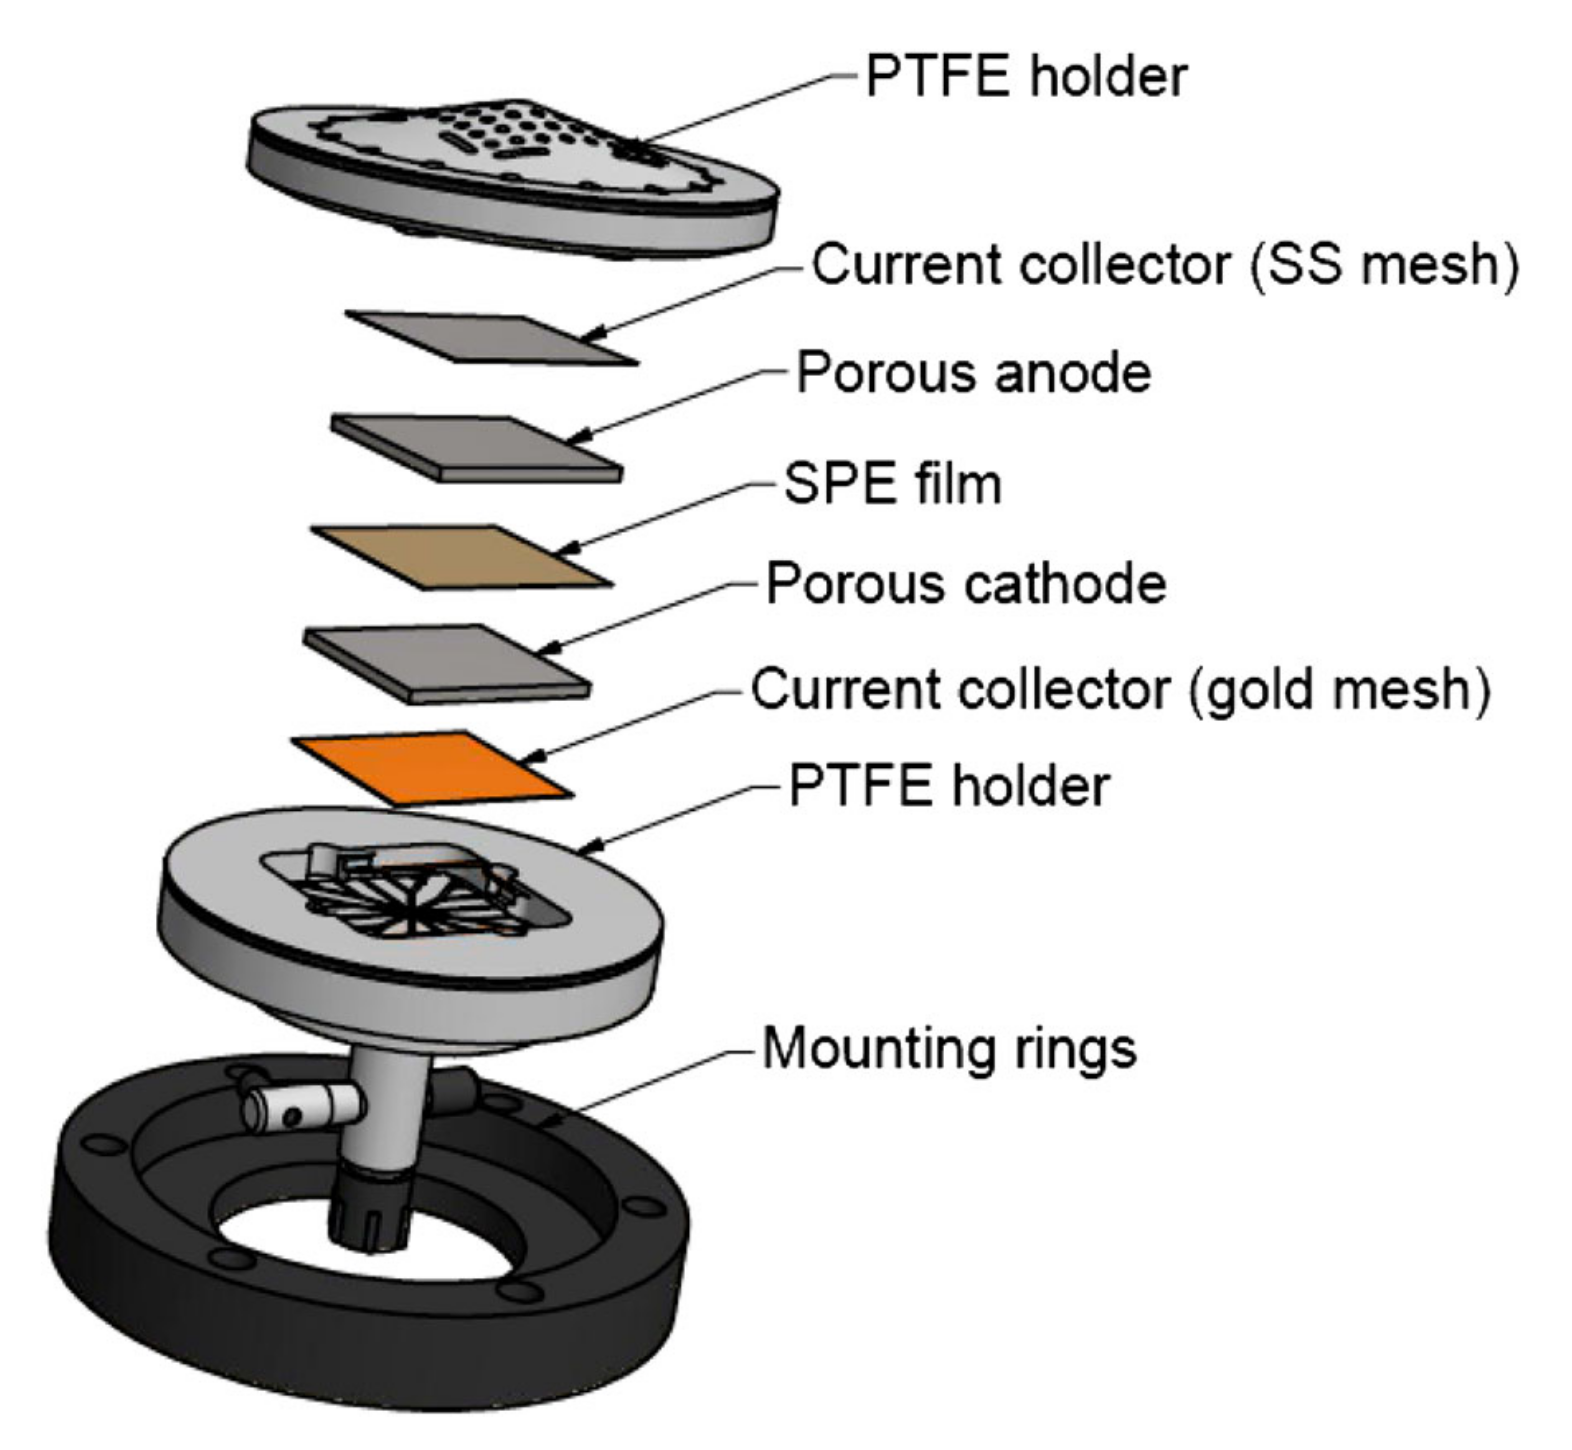
\includegraphics[width=0.6\linewidth]{PEM_cell_construction_elements.png}
    \caption{Sandwich parts arrangement}
    \label{fig:placeholder}
\end{figure}
 \item Align the engraved section of the bottom holder with one of the holes in the base mounting ring.
\end{itemize}

\begin{figure}[H]
    \centering

    \begin{subfigure}{0.45\textwidth}
        \centering
        \includegraphics[width=\linewidth]{20260819_101931.jpg}
        \caption{Sandwich before the MEA holder is closed}
        \label{fig:s5}
    \end{subfigure}
    \hfill
    \begin{subfigure}{0.45\textwidth}
        \centering
        \includegraphics[width=\linewidth]{Screenshot 2026-08-21 092609.png}
        \caption{The highlighted engraved part has to be aligned with one of the holes in the holder ring}
        \label{fig:s6}
    \end{subfigure}
\end{figure}

\begin{itemize}
    \item Insert six M6 screws through the top holder for subsequent attachment to the glass reservoir.

    \item Secure the top holder to the bottom holder and mounting ring using six M8 screws. Do not place washers between the top holder and bottom mounting ring.

    \item Tighten the screws uniformly, avoiding overtightening to prevent damage to the current collectors by the terminal wires.

    \item Leave the assembled sandwich submerged in the water bath for several hours.

    \item Remove the sandwich from the water bath and attach it to the glass reservoir using the six M6 screws. Place a seal ring between the reservoir and the sandwich.

    \item Attach the drain valve to the bottom of the sandwich.
\end{itemize}


\begin{figure}[H]
    \centering

    \begin{subfigure}{0.45\textwidth}
        \centering
        \includegraphics[width=\linewidth]{20260819_101241.jpg}
        \caption{The top holder}
        \label{fig:s7}
    \end{subfigure}
    \hfill
    \begin{subfigure}{0.45\textwidth}
        \centering
        \includegraphics[width=\linewidth]{20260819_101307.jpg}
        \caption{The assembled sandwich}
        \label{fig:s8}
    \end{subfigure}
\end{figure}

 

\subsubsection{The condenser }
\begin{itemize}
    \item Place a seal ring between the condenser and the upper end of the glass reservoir.

    \item Attach the condenser to the upper mounting ring using six M8 screws.

    \item Keep the glass reservoir supported on a stand during assembly to prevent damage to the electrical terminals.

    \item Using a manual tube bender, bend a 1/4-inch metal tube to the dimensions in  figure ~\href{fig:s10}{6b} to form the exhaust tube.

    \item Fit the exhaust tube with a Swagelok connector and attach it to the condenser.
\end{itemize}

\begin{figure}[H]
    \centering

    \begin{subfigure}{0.45\textwidth}
        \centering
        \includegraphics[width=\linewidth]{20260819_110319.jpg}
        \caption{Condenser with exhaust tube}
        \label{fig:s9}
    \end{subfigure}
    \hfill
    \begin{subfigure}{0.45\textwidth}
        \centering
        \includegraphics[width=\linewidth]{ChatGPT Image Sep 21, 2026, 11_00_26 AM.png}
        \caption{Sketch of exhaust tube with angles read on a manual tube bender}
        \label{fig:s10}
    \end{subfigure}
\end{figure}

Add an identity label to the PEM cell (this consist of the date the cell was assembled and cell number).

\subsubsection{Stack Assembly}
\newpage
\section{Operation of the electrolysis cell}
Add a  sample label (which consists of the date of start of the enrichment and sample number) to the empty PEM cell and weigh it. Remove the condenser top and add the required amount of sample water. Ensure there is no spillage. Weigh the sample. Do not include the mass of the stand when weighing the cell.
\begin{figure}[H]
    \centering

    \begin{subfigure}{0.45\textwidth}
        \centering
        \includegraphics[width=\linewidth]{20260911_103046.jpg}
        \caption{Weighing of the empty cell}
        \label{fig:s11}
    \end{subfigure}
    \hfill
    \begin{subfigure}{0.45\textwidth}
        \centering
        \includegraphics[width=\linewidth]{20260911_104520.jpg}
        \caption{Adding of the sample water}
        \label{fig:s12}
    \end{subfigure}
\end{figure}
Close the cell by putting back the condenser top then weigh and record the mass of the cell and sample water in a table such as \ref{tab:pem_enrichment_data}. Make sure to use the same screws and washers initially removed for mass consistency.

\begin{table}[H]
\centering
\caption{PEM enrichment data capture table}
\label{tab:pem_enrichment_data}

\renewcommand{\arraystretch}{1.6}

\resizebox{\textwidth}{!}{%
\begin{tabular}{|c|c|c|c|c|c|c|c|c|c|c|}
\hline

% Group headings
\multicolumn{3}{|c|}{} &
\multicolumn{5}{c|}{\textbf{Enrichment Start}} &
\multicolumn{3}{c|}{\textbf{Enrichment End}} \\
\hline

% Column headings
\textbf{Sample} &
\textbf{Cell ID} &
\textbf{Cell Beta} &
\textbf{Date} &
\textbf{Time} &
\begin{tabular}[c]{@{}c@{}}
\textbf{PEM Weight}\\
\textbf{Empty (g)}
\end{tabular} &
\begin{tabular}[c]{@{}c@{}}
\textbf{PEM Weight}\\
\textbf{Full (g)}
\end{tabular} &
\begin{tabular}[c]{@{}c@{}}
\textbf{$M_1 =$ H$_2$O}\\
\textbf{Weight (g)}
\end{tabular} &
\textbf{Date} &
\textbf{Time} &
\begin{tabular}[c]{@{}c@{}}
\textbf{PEM Weight}\\
\textbf{Final (g)}
\end{tabular} \\
\hline

% Empty row 1
\rule{0pt}{1.2cm} & & & & & & & & & & \\
\hline

% Empty row 2
\rule{0pt}{1.2cm} & & & & & & & & & & \\
\hline

% Empty row 3
\rule{0pt}{1.2cm} & & & & & & & & & & \\
\hline

% Empty row 4
\rule{0pt}{1.2cm} & & & & & & & & & & \\
\hline

% Empty row 5
\rule{0pt}{1.2cm} & & & & & & & & & & \\
\hline

\end{tabular}%
}
\end{table}
\subsection{Running the electrolysis}
From a central laptop, open the terminal and log in with ssh water@pem-chicken (to log into chicken). This attaches to a persistent screen session on the Raspberry Pi so pemcell keeps running if the connection drops.
Enter; Run pemcell, to start

Follow the interactive prompts:
\begin{itemize}
    \item Enter sample name (Label for this run, use the date and sample number )
    \item Zero load cell; remove PEM cell from load cell, press ENTER
    \item Calibrate load cell; install full PEM cell (without wires) with known weight; enter weight in grams
    \item Attach wires ; Connect wires from PEM and cooler top to power supplies; press ENTER so wire weight is included in process control.
    \item Enter water amount — grams of water in PEM cell
    \item Start — Press ENTER to begin electrolysis
    \item Record the date and time of the start of electrolysis.
Electrolysis — Runs until water target weight is reached (in this case 20g). Log file name is shown on screen; process information is displayed on screen, and saved to the log file. Press ENTER to pause (or stop) the electrolysis. Weigh and record the PEM cell after electrolysis in table \ref{tab:pem_enrichment_data}.
\end{itemize}
\subsection{Post enrichment processes}
\subsubsection{Cold trap extraction}
Weigh the empty cold trap ( do this by switching on the pump, then close the inlet of the trap with Swagelok valve, wait about 30 seconds, then close the outlet. 
\begin{figure}[H]
    \centering

    \begin{subfigure}{0.45\textwidth}
        \centering
        \includegraphics[width=\linewidth]{20260916_132127.jpg}
        \caption{Weighing of the empty extraction tube}
        \label{fig:s13}
    \end{subfigure}
    \hfill
    \begin{subfigure}{0.45\textwidth}
        \centering
        \includegraphics[width=\linewidth]{20260910_162116.jpg}
        \caption{PEM cell connected to the extraction system}
        \label{fig:s14}
    \end{subfigure}
\end{figure}







Connect the trap and the PEM cell to the extraction system. Note the date and time for the start of the extraction. Switch on the heating pan and set the temperature to $50 \degree\text{C}$. Make sure all the Swagelok valves are open. Open the drain valve of the PEM cell slowly. Dip the extraction tube in a flask filled with liquid nitrogen to condense extracted sample. Place a heat gun at 4cm from the Swagelok inlet valve and set it on to a temperature of $100 \degree\text{C}$ . Turn on the vacuum pump and slowly increase the suction up to mid-level. Keep adding liquid nitrogen every 20-30 minutes or when the level decreases.
\begin{figure}[H]
    \centering

    \begin{subfigure}{0.45\textwidth}
        \centering
        \includegraphics[width=\linewidth]{20260910_162023.jpg}
        \caption{Heating pan set to 50 degrees celsius}
        \label{fig:s15}
    \end{subfigure}
    \hfill
    \begin{subfigure}{0.45\textwidth}
        \centering
        \includegraphics[angle=-90,origin=c,width=\linewidth]{20260910_164422.jpg}
        \caption{Heat gun set to level II, 100 degrees celsius and placed 4cm from the swagelok valve}
        \label{fig:s16}
    \end{subfigure}
\end{figure}

Keep the extraction going for about 2-3 hours. At the end of  extraction, close the inlet of the cold trap, wait a few seconds and close the outlet of the cold trap. Let the extraction tube sit overnight to warm up to room temperature on its own. Weigh the PEM cell and the extraction tube at the end of extraction and record the data in table \ref{tab:cold_trap_extraction}.  

\begin{table}[H]
\centering
\caption{Cold trap extraction data}
\label{tab:cold_trap_extraction}

\renewcommand{\arraystretch}{1.6}

\begin{tabular}{|c|c|c|c|c|}
\hline

\multicolumn{5}{|c|}{\textbf{Cold Trap Extraction}} \\
\hline

\textbf{Start Time} &
\textbf{End Time} &
\begin{tabular}[c]{@{}c@{}}
\textbf{Trap Weight}\\
\textbf{Empty (g)}
\end{tabular} &
\begin{tabular}[c]{@{}c@{}}
\textbf{Trap Weight}\\
\textbf{Full (g)}
\end{tabular} &
\begin{tabular}[c]{@{}c@{}}
\textbf{H$_2$O Weight}\\
\textbf{(g)}
\end{tabular} \\
\hline

\rule{0pt}{1.2cm} & & & & \\
\hline

\rule{0pt}{1.2cm} & & & & \\
\hline

\rule{0pt}{1.2cm} & & & & \\
\hline

\rule{0pt}{1.2cm} & & & & \\
\hline

\rule{0pt}{1.2cm} & & & & \\
\hline

\end{tabular}
\end{table}
 

\subsection{Vial Transfer}
Add a label to the cap of the vial (this consists of the date in the format YYMMDD and a letter for sample number e.g 261015A ) . Weigh and record the mass of the empty vial then zero the scale. 
(do not write anything to the container vial as it may interfere with scintillation processes)

\begin{figure}[H]
    \centering

    \begin{subfigure}{0.45\textwidth}
        \centering
        \includegraphics[angle=-90,origin=c,width=\linewidth]{20260918_144922.jpg}
        \caption{Weighing of the empty vial}
        \label{fig:s17}
    \end{subfigure}
    \hfill
    \begin{subfigure}{0.45\textwidth}
        \centering
        \includegraphics[angle=-90,origin=c,width=\linewidth]{20260918_145304.jpg}
        \caption{Pipette with tube for single use transfer of sample to vial}
        \label{fig:s18}
    \end{subfigure}
\end{figure}



Use a pipette to carefully add about 8 ml of the enriched sample water to the vial. Ensure that there is no spillage. Weigh and record the mass the sample water. Add 2 x 6 ml of scintillation cocktail. Weigh and record the mass of the scintillation cocktail.  
\begin{figure}[H]
    \centering

    \begin{subfigure}{0.45\textwidth}
        \centering
        \includegraphics[angle=-90,origin=c,width=\linewidth]{20260918_145823.jpg}
        \caption{Weighing of the sample}
        \label{fig:s19}
    \end{subfigure}
    \hfill
    \begin{subfigure}{0.45\textwidth}
        \centering
        \includegraphics[angle=-90,origin=c,width=\linewidth]{20260918_145949.jpg}
        \caption{Weighing of the cocktail}
        \label{fig:s20}
    \end{subfigure}
\end{figure}


Ensure the cap of the vial is tightly closed. Record the mass of the sample on the cap. Dispose of the pipette tube before transferring a new sample. Store the vials in a cool dry and dark place . Clean and dry the cold trap and conical flask set-up before the next extraction.

\subsection{Sample Measurement with LSC}

\end{document}
